% !TeX root = ../Praktikum.tex
\section{FPGA-basierte Bildanalyse und Dimming-Algorithmus}
\label{sec:PROJEKT}

%auf SPI Mode löten
%Stecker Modifikation wie DEMO (siehe Bilder)
	%orig. VCC weg
	%VCC an SDO
	%orig. SDO trennen 

%an JC PMOD vom Digilent Board (siehe Bilder)
%VCC Ausrichtung beachten



In diesem zweiten Versuch des Mikroelektronik Praktikums wird ein LC-Displays mit einem FPGA angesteuert. Hierbei wird das Interface für eine einfache, serielle Kommunikation zur Verfügung gestellt. Im Folgenden wird das verwendete Display beschrieben. Insbesondere wird auf die vom Display\footnote{genau genommen ist hier der Controller gemeint, welcher auf dem PCB des Displays sitzt und die Daten annimmt} entgegengenommenen Befehle und deren Umsetzung im FPGA eingegangen.\\
Das Ziel des Projektes, ist es einen Global-Dimming Algorithmus auf einer Pixelpipeline ohne der Verwendung von Framebuffern im FPGA zu implementieren und auf einem Display zu validieren. Der zu implementierende Algorithmus wird in Kapitel \ref{subsec:funktion_global_dimming} erläutert. Zunächst wird jedoch auf das verwendete Display eingegangen.

\subsection{Beschreibung des verwendeten Displays}
\label{subsec:Display_Beschreibung}
Für dieses Praktikum wird ein LC-Display der Firma \emph{Digole}\cite{digole}verwendet. Hierbei handelt es sich um ein Active-Matrix IPS-Panel mit einer Auflösung von 240RGBx320 Pixeln und einer Display-Diagonalen von 2,6 Zoll. Das Display wurde für den Einsatz an Mikrocontrollern entwickelt, weshalb es mehrere serielle Datenübertragungsprotokolle unterstützt. Um die schnellste Datenübertragung zwischen FPGA und Display zu gewährleisten wurde für dieses Praktikum eine Übertragung der Bilddaten mittels SPI gewählt. Das verwendete Display ist in Abbildung \ref{fig:display} dargestellt.
\begin{figure}[H]
\centering
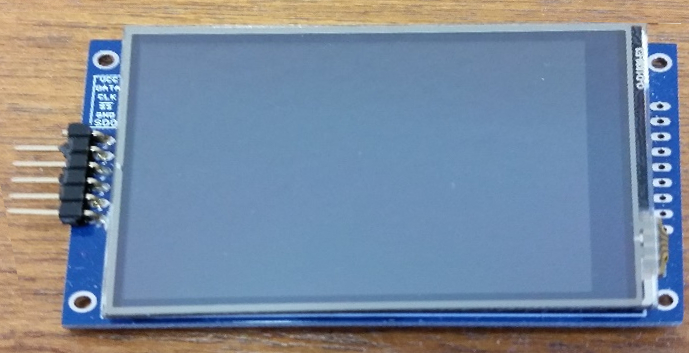
\includegraphics[width=0.5\linewidth]{img/display_projekt/display}
\caption{Für diese Praktikum verwendetes Display}
\label{fig:display}
\end{figure}

Zur Ansteuerung dieses Displays wird das bereits bekannte FPGA-Board Basys 2 von Digilent\cite{basys2} eingesetzt. Da die Pin-Belegung der PMOD-Ausgänge des FPGA-Boards bei den VCC und GND-Pins nicht mit der Belegung des Displays im Originalzustand übereinstimmen, wurden die Pins am Display so manipuliert, dass eine Verwendung am PMOD Ausgang des FPGAs möglich ist. Hierzu wurde der ursprüngliche VCC-Pin des Displays entfernt und der Anschluss an der Rückseite des Displays mit dem ursprünglichen SDO-Pin verbunden. Die SDO Verbindung zum Display selbst wurde hierbei natürlich ebenfalls unterbrochen, da diese für die SPI-Kommunikation auch nicht notwendig ist. Der Modus für den SPI-Betrieb kann auf der Display Rückseite durch Jumper bzw. Löten eingestellt werden.\\
Dadurch ist es möglich, die Power-Supply des Basys 2 zu nutzen ohne eine eigene Power-Supply für das Display betreiben zu müssen. Auch die Kommunikation zwischen FPGA und Display funktioniert, wenn das bearbeitete Display an einem PMOD des Basys 2 angeschlossen und das FPGA mit dem entsprechendes Bitfile programmiert wird. Dies ist in Abbildung \ref{fig:display_bespiel_angeschlossen} nochmal dargestellt. 
\begin{figure}[H]
\centering
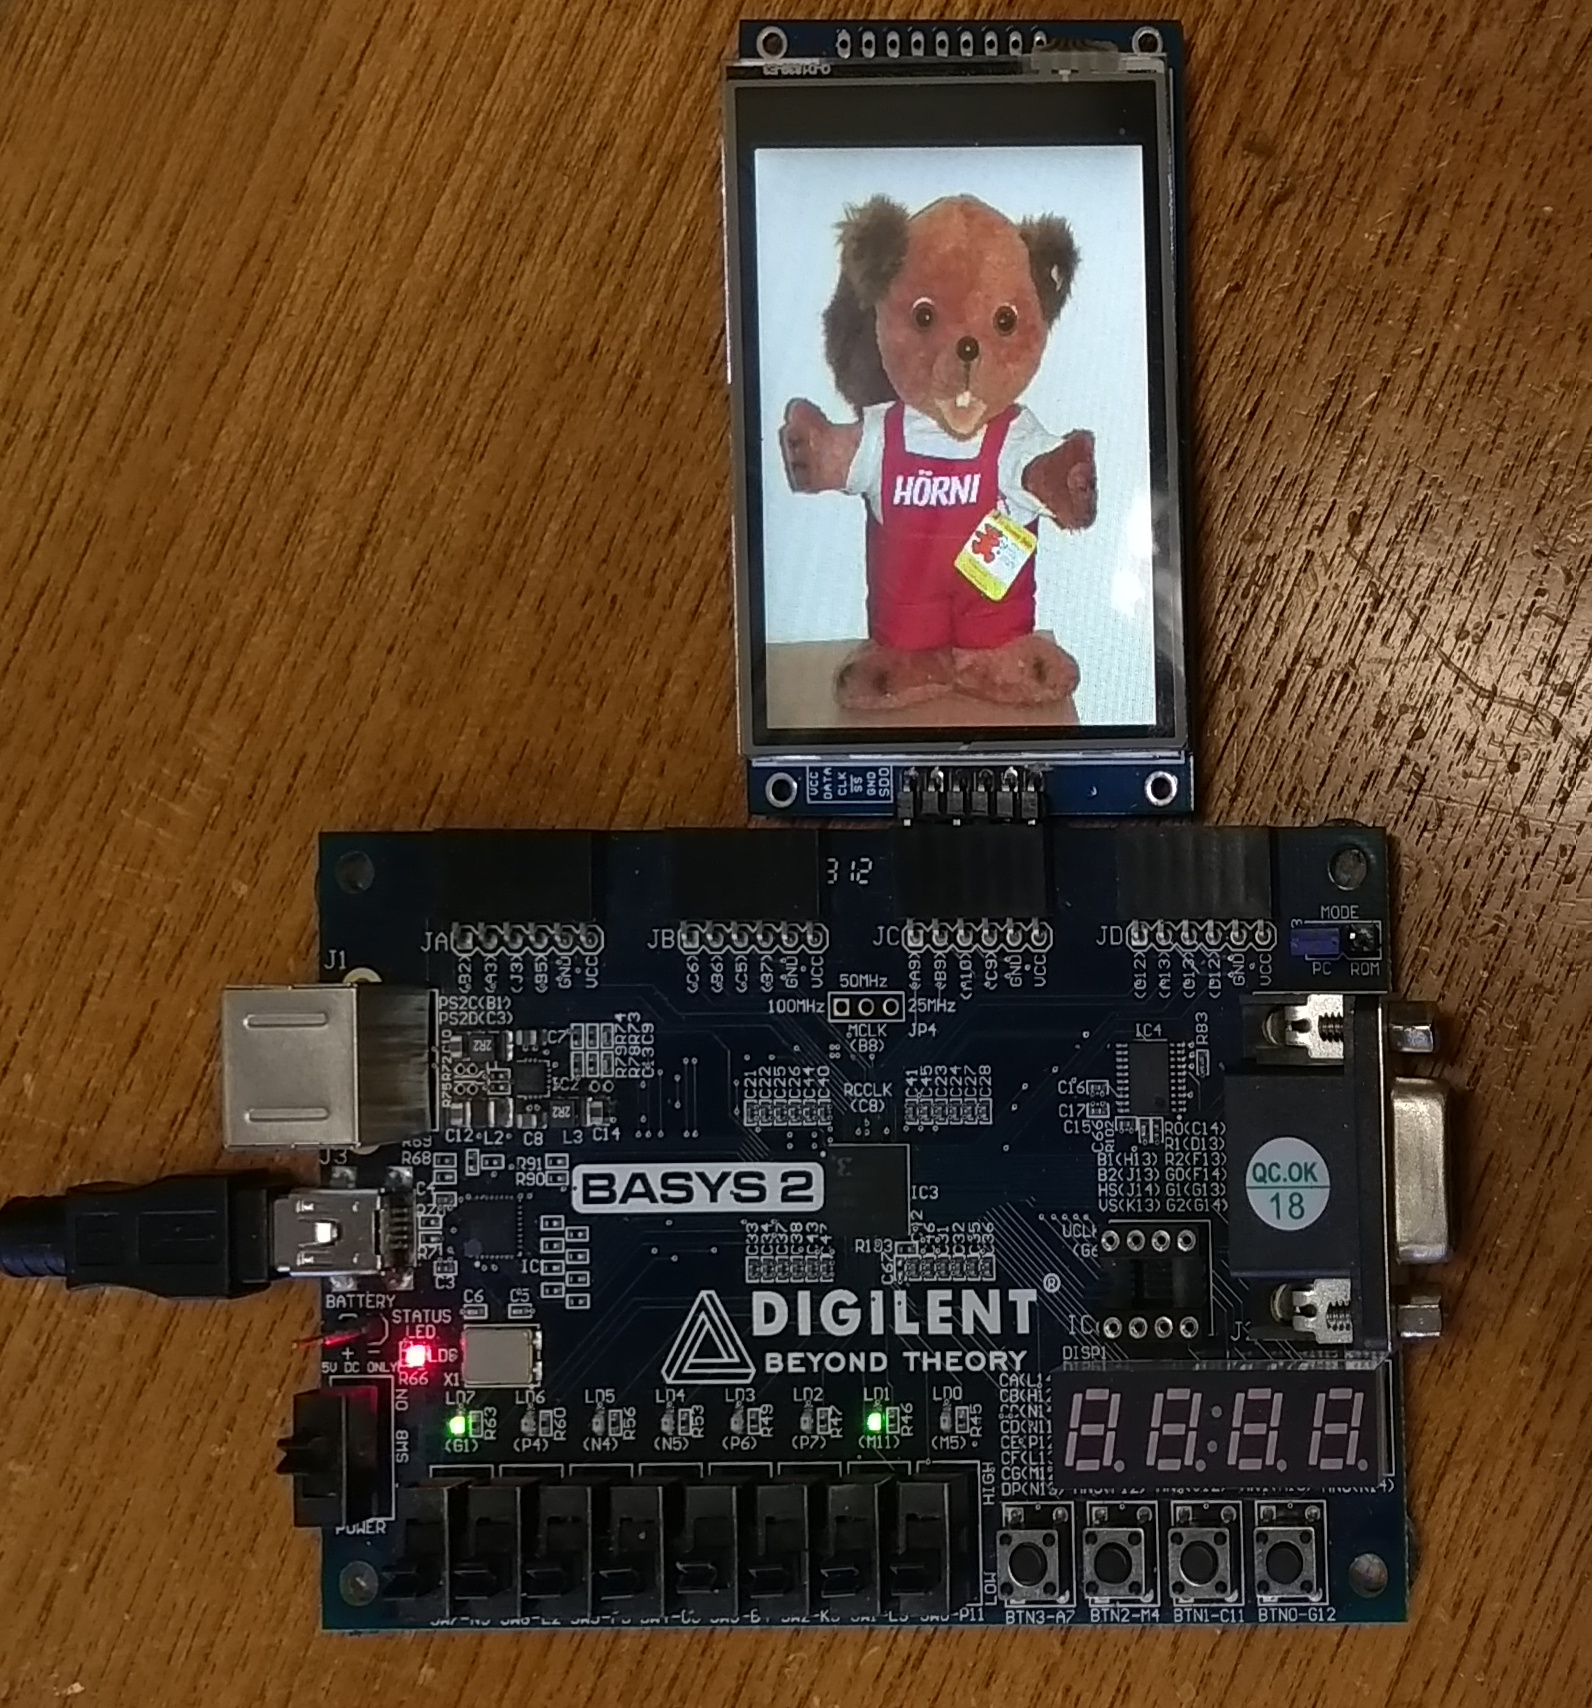
\includegraphics[width=0.8\linewidth]{img/display_projekt/display_bsp_fpga}
\caption{Basys 2 Board mit angeschlossenem Display an einem PMOD.}
\label{fig:display_bespiel_angeschlossen}
\end{figure}
Da das verwendete Display über ein vereinfachtes Interface verfügt, welches zwar für Mikrocontroller leicht umzusetzen, in FPGAs aber aufwendig zu realisieren ist, wird das serielle SPI Interface in Verilog für dieses Praktikum vorgegeben. Dieses vereinfachte Interface (durch den Display-Timing-Controller, \emph{TCON} realisiert) übernimmt die eigentliche Ansteuerung der TFT-Matrix des Displays.\\
Im Folgenden wird kurz die Funktionsweise dieses Interfaces erläutert und erklärt, weshalb dies im FPGA zu Schwierigkeiten führt. 
Die Kommunikation mit dem Display basiert hierbei stets auf der seriellen Übertragung einzelner Bytes. Dabei ist es nicht von Bedeutung, mit welchem Protokoll dieses Byte übertragen wird. Der Einfachheit und höherer Geschwindigkeit halber, wurde hier eine SPI-Übertragung gewählt.
Dank der Funktionsvielfalt des Displaycontroller, ist es durch das Übertragen einzelner Bytes für einen Mikrocontroller einfach, auch komplexe Zeichen, wie z.B. auch Buchstaben und Symbole direkt auf dem Display anzuzeigen oder Befehle zum rendern an das Display zu senden.\\
Im FPGA hingegen muss zunächst ein spezielles Modul für die SPI-Übertragung implementiert und auch korrekt seriell mit den entsprechenden Bytes in einem Zustandsautomaten angesteuert werden. Im Praktikum jedoch soll auf einer Pixel-Pipeline gearbeitet werden. Dies bedeutet, dass das Display das darzustellende Bild pixelweise erhalten soll. Aus diesem Grund wird das Display im sogenannten \emph{Video-Mode} betrieben. Das Display wechselt in diesen Modus, nachdem es nacheinander die Zeichen\footnote{Zeichen entsprechen binären Werten. Siehe ASCII.} `V', `I', `D', `E', `O' übermittelt bekommt. Dieser Befehl wird gefolgt von der Auflösung und der Startposition des auszufüllenden Rechtecks. Im Anschluss kann genau die Anzahl an Pixelwerten übertragen werden wie in dem vorherbestimmten Rechteck vorhanden sind. Danach wird der Video-Modes automatisch wieder verlassen. Da es leider nicht möglich ist, alle Pixel des Displays mit einem einmaligen Aufruf des Video-Modes zu bespielen, wurde nach der Hälfte der Zeilen ein zweiter Video-Mode aufgerufen. Dies ist beim Bildaufbau deutlich an der kurzen Pause an dieser Stelle zu erkennen (siehe Abbildung \ref{fig:display_bespiel_video_mode}). Zusätzlich zu diesem erläuterten Modus, kann noch ein globaler PWM-Wert übermittelt werden, um das Backlight anzupassen.
\begin{figure}[H]
\centering
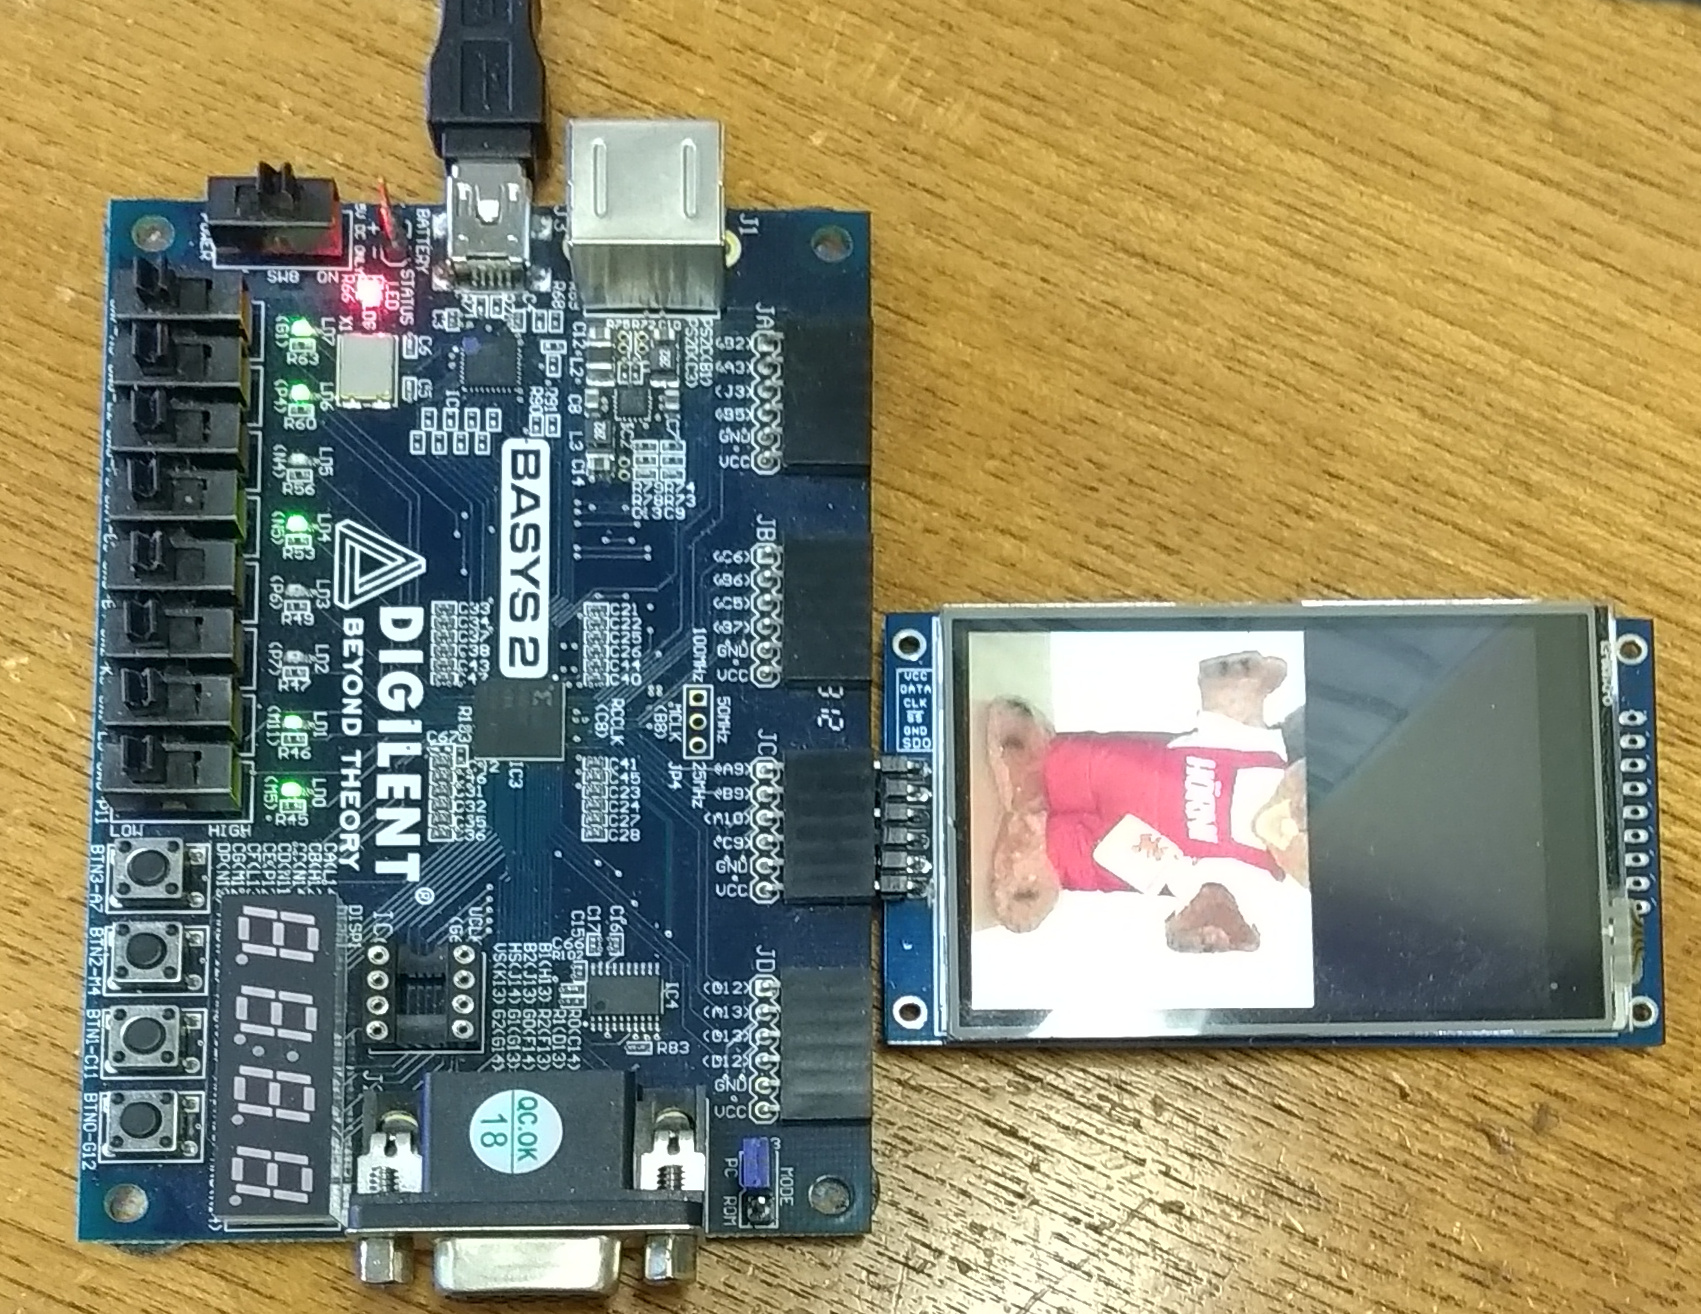
\includegraphics[width=0.8\linewidth]{img/display_projekt/display_video_mode}
\caption{Display beim Bildaufbau. Start der zweiten ``Video-Box''.}
\label{fig:display_bespiel_video_mode}
\end{figure}
Zur seriellen Übertragung der Bilddaten an das Display wird eine Blackbox bzw. Modul bereitgestellt, welche diese Video-Modes initiiert und die Bilddaten (siehe Kapitel \ref{subsec:datenuebertragung}) über ein Protokoll welches die USB-Verbindung mit dem Board nutzt, annimmt und auch per SPI an das Display überträgt. Dies führt dazu, dass ein Algorithmus von Ihnen leicht ohne tiefere Kenntnis der SPI-Kommunikation integriert werden kann. Das genannte Modul stellt außerdem die von einem PC gesendeten Bilddaten in einer Pixel-Pipeline zur Verfügung. So ist es einfach möglich, die in diesem Versuch behandelten Algorithmen mit Hilfe des vorhandenen Interfaces zu implementieren und zur Blackbox weiterzuleiten. Das gesamte Grundgerüst wird in Kapitel \ref{subsubsec:Beschreibung_vorhandenes_Verilog_Modul} beschrieben.\\
Doch zunächst wird im nächsten Abschnitt die Datenübertragung vom PC zum FPGA behandelt.
\subsection{Datenübertragung vom PC zum FPGA}
\label{subsec:datenuebertragung}
%%ISE Projekt. Studenten bekommen TOP, UCF,senden_modul, und Dimming Modul IOs bzw. als Durchschleif 
%Bytestream-Generierungsfile mk_image_bit.m generiert Bit-/Bytestream data.bin mit kodierter Pixelclock im LSB
%An Studenten wird der Ordnerinahlt Matlab/Bitstream_Generierung_aus_Bild/pcode/ zur Verfügung gestellt
%later: wenn alles läuft soll die DEPP Kommunikation über Matlab laufen (SDK mit C-Code existiert) 

Da der interne Speicher des FPGAs nicht ausreicht, um ein komplettes Bild mit der Auflösung von 320x240 Pixeln bereits im Bit-File bei der Programmierung des FPGAs zu speichern, ist es erforderlich, die Bilddaten von einem PC zur Laufzeit zum FPGA zu übertragen und eine Pixel-Pipeline zu erzeugen. \\
Als schnelle Übertragung bietet sich hier das von Digilent unterstützt \emph{DEPP} Protokoll an. Mit diesem Protokoll können ganze Dateien mit der von Digilent entwickelten Adept Software (bzw. deren API) in einfacher Weise vom PC zum FPGA übertragen werden. Für diese Übertragung, muss zunächst ein Bytestream in Matlab aus dem gewünschten anzuzeigenden Bild generiert werden. Für die Generierung wird eine Matlab Funktion zur Verfügung gestellt und befindet sich im Ordner\\
\texttt{\centerline{\netzwerkpfadSource/Bitstream\_Generierung\_aus\_Bild/pcode/}}\\
auf dem Netzlaufwerk und wird im nächsten Abschnitt erläutert.\\
Dabei ist zu beachten, dass das unten aufgeführte Programm \emph{Ausführungsrechte} (\emph{execute}) auf dem Dateisystem hat. Die Übertragung (entsprechendes Bit-File vorausgesetzt) kann mit
\begin{center}
\texttt{./DeppCommunication -l 0 -d Basys2 -f data.bin -c 1420800}
\end{center}
gestartet werden. Dabei ist \texttt{data.bin} die erzeugte Bytestream-Datei. Da die Übertragungsgeschwindigkeit vom PC und dessen Treiber abhängt, ist eine Synchronisation der ankommenden Daten auf dem FPGA mit den ausgehenden Daten über SPI an das Display erforderlich. Dies ist umso wichtiger, wenn bedacht wird, dass kein einziger Pixel im FPGA außerhalb der Pixel-Pipeline zwischengespeichert wird.

\subsubsection*{Generierung der Bytestream-Datei}
Um die Datei zu erstellen, welche wie oben beschrieben zum FPGA gesendet wird, soll eine Matlab Funktion verwendet werden. Mithilfe dieser Funktion kann eine beliebige Bilddatei mit einer Auflösung von 320x240 Pixeln eingelesen werden. Die einzelnen Pixel werden dann von der Funktion in eine entsprechende \emph{*.bin} Datei geschrieben. Die Signatur und Funktionsweise der Funktion kann aus Abbildung \ref{code:signatur_bytestream} entnommen werden.
Hierbei werden hintereinander jeweils alle RGB-Werte einzeln geschrieben. Um zu gewährleisten, dass die Übertragung des Streams vom PC zum FPGA nicht schneller abläuft als die Übertragung vom FPGA zum Display (-Controller) wird in diesem Beispiel jeden Pixel 4-mal in dem Stream gespeichert. Da das Display nur eine begrenzte Farbtiefe (Daten) entgegennimmt, wird das LSB genutzt, um eine künstliche bzw. virtuelle Pixelclock zu generieren, welche es erlaubt, die Daten zwischen FPGA und PC zu synchronisieren. Die resultierende Datenstruktur ist in der folgenden Tabelle \ref{tab:bytestream} dargestellt. \\
Hierbei muss auf jeden Fall sichergestellt werden, dass die Übertragung zum FPGA langsamer ist als die Übertragung vom FPGA zum Display. Da im FPGA kein Zwischenspeicher vorhanden ist, würden dann direkt Pixelwerte und somit Daten verloren gehen und es kommt zu Lücken im anzuzeigenden Bild. 
\begin{figure}[H]
	\lstset{style=matlab-style}
\begin{lstlisting}
%  GENERATE_IMAGE_BIT_FUN Generates the Bitstream for a given image
%    RES = GENERATE_IMAGE_BIT_FUN(IMAGE,FILENAME_OUT) resizes IMAGE to a
%    resolution of 320x240 (ROWSxCOLS) and stores the bytestream
%    to FILENAME_OUT which can be used to be transmitted to the FPGA.
%    
%    IMAGE should be of UINT8 type (matrix, RGB).
% 
%    For more information consider to ask Tim Goll.
%    
%    See also UINT8.
%
\end{lstlisting}
\label{code:signatur_bytestream}
\caption{Funktionsbeschreibung der gegeben MATLAB-Funktion}
\end{figure}


\begin{table}[h]
	\begin{center}
	 \rowcolors{2}{white}{lme2}
		\begin{tabular}{c l c}
		\hline
		\textbf{MSB} & & \textbf{LSB}\\
		\hline		\hline
		NN & \textbf{X} Bit Rot & 0\\
		NN & \textbf{X} Bit Rot & 0\\
		NN & \textbf{X} Bit Rot & 0\\
		NN & \textbf{X} Bit Rot & 0\\	
		NN & \textbf{X} Bit Grün & 1\\								
		NN & \textbf{X} Bit Grün & 1\\			
		NN & \textbf{X} Bit Grün & 1\\								
		NN & \textbf{X} Bit Grün & 1\\	
		NN & \textbf{X} Bit Blau & 0\\								
		NN & \textbf{X} Bit Blau & 0\\						
		NN & \textbf{X} Bit Blau & 0\\						
		NN & \textbf{X} Bit Blau & 0\\ 			
		NN & usw. ... & usw. ...\\																									
		\hline
		\end{tabular}
		\caption{Aufbau und Struktur des Bytestreams}
		\label{tab:bytestream}
	\end{center}
\end{table}
Zu Beginn der Bytestream-Datei werden zunächst einige 0-Werte geschrieben, da die Zeit, welche die Übertragung dieser 0-Werte benötigt ausreicht, um eine Video-Box im Display zu initialisieren. Das FPGA beginnt mit dem Initialisierungsvorgang, sobald der erste Wert mit Hilfe des EPP Protokolls entgegengenommen wird. Die gleiche Delay-Phase existiert in der Mitte des Streams, da zu diesem Zeitpunkt, wie bereits oben beschrieben, eine zweite Video-Box initiiert werden muss. 
 


\subsection{Display Timing und Pixel-Pipeline im Allgemeinen}
\label{subsec:display_timing}
Bei höheren Auflösungen reicht die SPI-Schnittstelle nicht aus, um flüssige Bilderfolgen darzustellen. So existiert beispielsweise die Standardisierungsorganisation \emph{Video Electronics Standards Association} oder kurz \emph{VESA}, welche für die Spezifizierung von Videostandards zuständig ist. Ein Beispiel eines Timings sei in Abbildung \ref{fig:display_timing_bespiel} gegeben. Weitere Timings sind in \cite{vesa_timing} zu finden.
\begin{figure}[H]
\centering
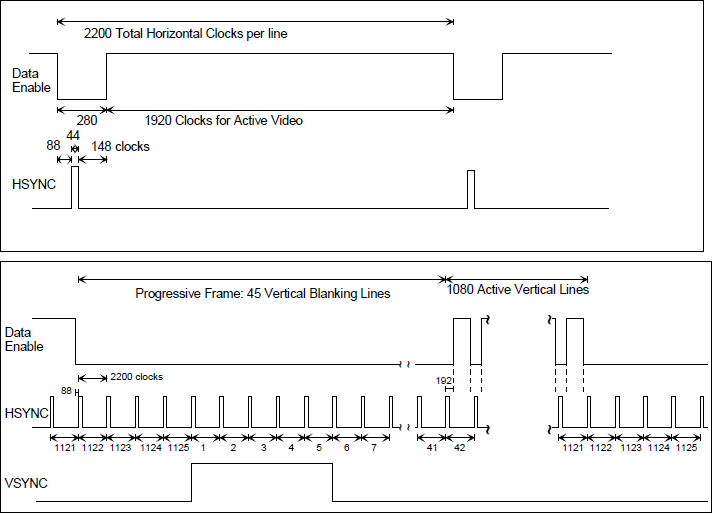
\includegraphics[width=0.8\linewidth]{img/display_projekt/timing_allgemein_beispiel_mod}
\caption{Beispiel des Timings eines Displays}
\label{fig:display_timing_bespiel}
\end{figure}
Die Signale \emph{HSYNC} und \emph{VSYNC} können sowohl active-high als auch active-low sein. Sie sind noch historische Überbleibsel der analogen Videoübertragung und Darstellung auf einem Röhrenbildschirm. HSYNC ist in der horizontalen \emph{Blanking}-Zeit für einen spezifizierten Zeitanteil aktiv und VSYNC entsprechend in der vertikalen \emph{Blanking}-Zeit. Die eigentliche Bilddaten sind während der \emph{Data Enable} high-Phase gültig. Dabei sind die Subpixel parallel verfügbar. Die Pixelclock, welche gerade den Takt der RGB-Pixel beschreibt, wird in Hardware verwendet, um synchron zu der Pixel-Pipeline arbeiten zu können.\\
Zur Kommunikation zwischen mehreren ICs wurde (und wird immer noch) der \emph{ Flat-Panel-Display (FPD)} Link verwendet, welcher auf dem differentiellen Verfahren \emph{Low Voltage Differential Signaling} kurz \emph{LVDS} basiert. Moderner ist das \emph{V-by-One} Verfahren (ebenfalls differentiell) von THine Electronics, welches längere Distanzen überbrücken kann und weitere Vorteile bietet. Zwischen Geräten sind die Schnittstellen \emph{High Definition Multimedia Interface}, kurz \emph{HDMI} sowie \emph{DisplayPort} geläufig.\\


\subsection{Global-Dimming Algorithmus}
\label{subsec:funktion_global_dimming}
Wie bereits in Kapitel \ref{sec:einleitung} erläutert, bieten Dimming-Algorithmen für LCDs effektive Möglichkeiten den Schwarzwert und Kontrast sowie die Powerconsumption zu verbessern. Es wird zwischen Local- und Global-Dimming unterschieden. Local-Dimming hat eine deutlich höhere Komplexität und erfordert eine komplexere Realisierung in Hardware, da hier die einzelnen LED Stränge einzeln gedimmt werden können und der Beitrag jedes Stranges zu jedem Pixel berücksichtigt werden muss. Andererseits liefert Local-Dimming bessere Resultate als Global-Dimming, welches auch 0D-Dimming genannt wird. Dabei werden alle vorhandenen LEDs auf einen gemeinsamen Faktor gedimmt. Der individuelle Leuchtdichtebeitrag der LEDs spielt in diesem Fall keine Rolle.\\
In diesem Praktikum soll so ein vereinfachter Global-Dimming-Algorithmus in einem FPGA auf einer virtuellen Pixelpipeline realisiert werden. Dabei wird kein Framebuffer verwendet. Zunächst wird die generelle Funktionsweise eines Global-Dimming Algorithmus nach dem Stand der Technik beschrieben
\subsubsection{State-of-the-Art Global-Dimming}
\label{subsub:SoA_0D}
Ein Global-Dimming-Verfahren beruht auf der Manipulation der Gammakurve. Es wird ein sogenannter Knickpunkt \emph{Q} in der Gammakurve eingeführt, ab dem sich der ursprüngliche Verlauf der Gammakurve ändert. So kann z.B. die Steigung der original Gamma-Kurve ab Q abgeflacht werden, so dass die maximale Leuchtdichte nicht mehr erreicht wird. In Abbildung \ref{fig:dimming_gamme_curve} wird solch ein Vorgehen exemplarisch dargestellt. Falls die ursprünglichen Grauwerte den maximal möglichen Wert angenommen hatten, ergibt sich hier ein Powersaving von 20\ \%.
\begin{figure}[H]
	\centering
	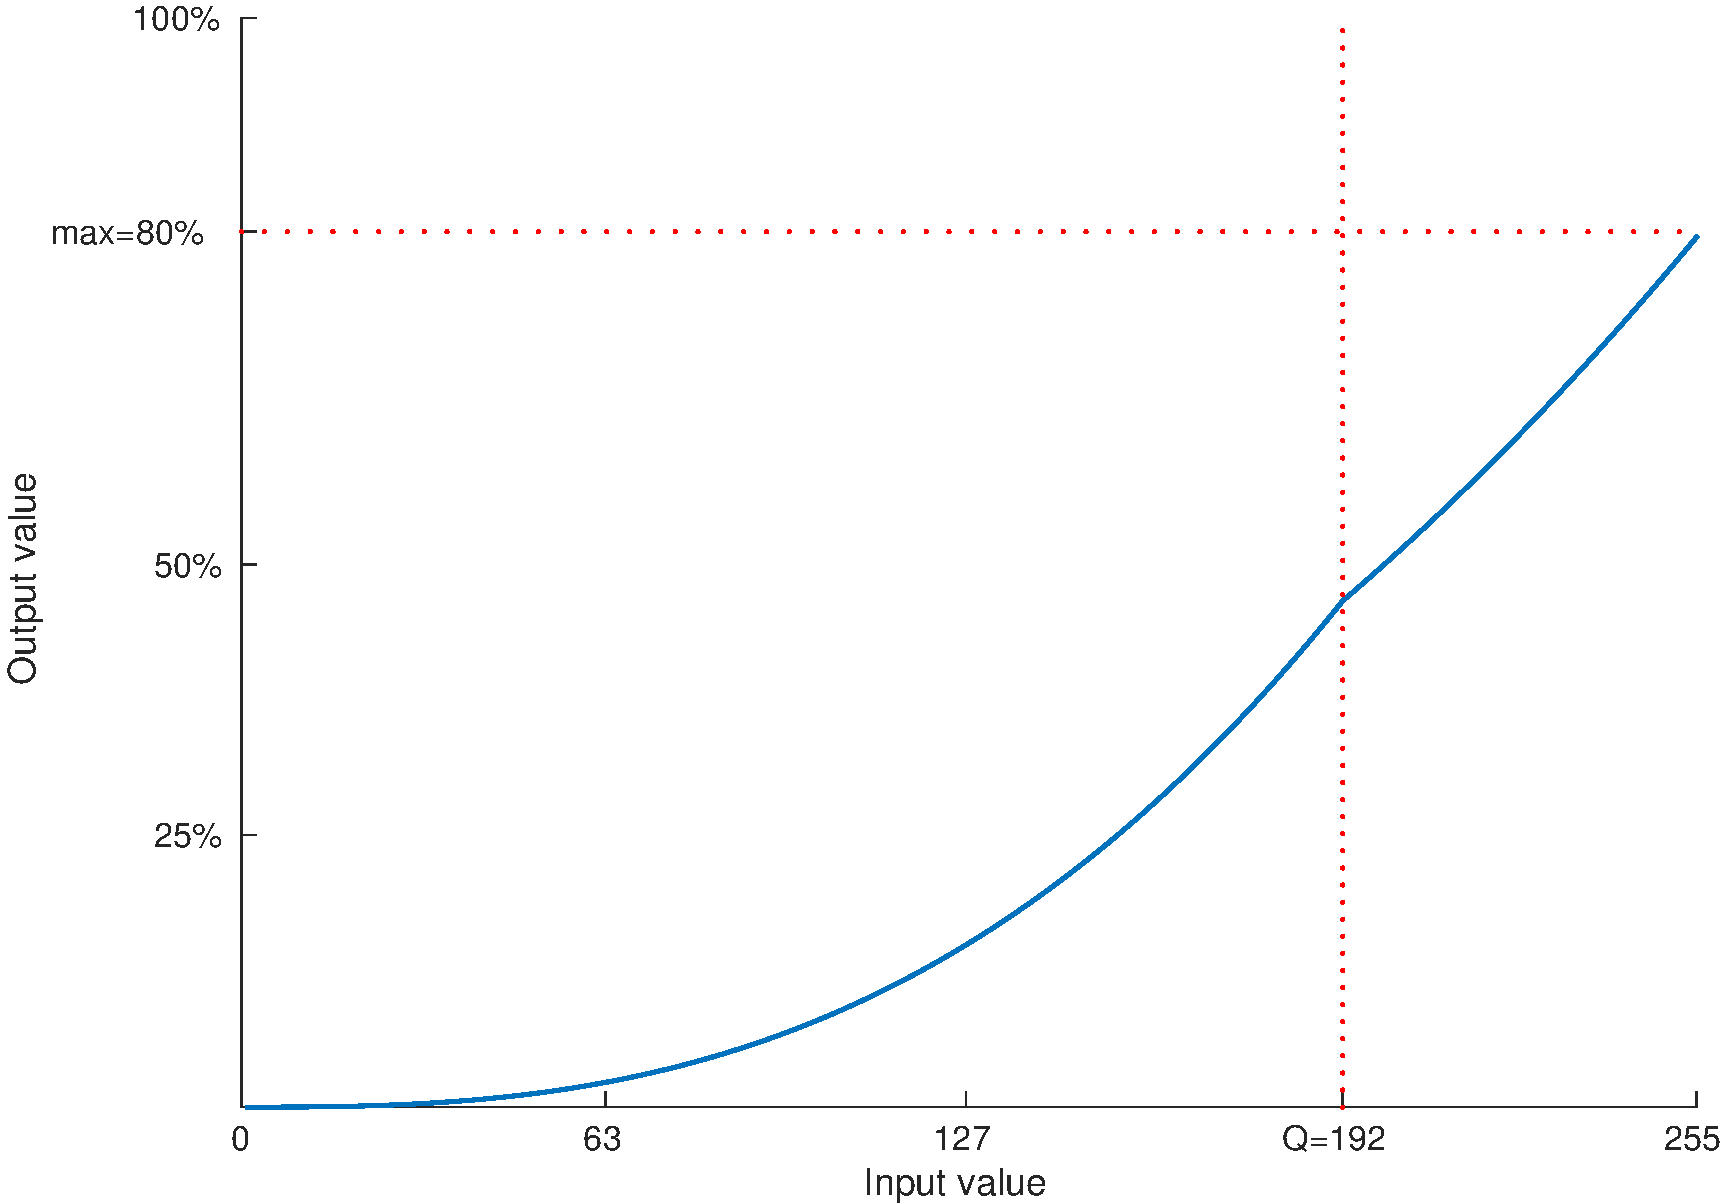
\includegraphics[width=0.6\linewidth]{img/display_projekt/0D_basics/mapping_curve_gamma_percent}
	\caption{Global-Dimming Funktionsprinzip \cite{Schmidt_edC16}}
	\label{fig:dimming_gamme_curve}
\end{figure}
Wird in diesem Fall das Backlight auf 80\ \% des ursprünglichen Wertes gedimmt, so erscheint das Bild insgesamt auch \emph{dunkler}. Um dies zu vermeiden, werden die Pixelwerte, nachdem das berechnete Backlight bekannt ist, \emph{kompensiert}. Das bedeutet, die \emph{Transmission} der einzelnen Pixel wird \emph{erhöht} um den Helligkeitsverlust des verringerten Backlights so weit wie möglich zu kompensieren. Mathematisch lässt sich die Kompensation für alle Pixel $ (i,j) $ wie folgt berechnen \cite[p.67]{Albrecht2010}:
\begin{equation}
\mathrm{p}^{\mathrm{comp}}_{i,j} = \mathrm{min}\left(\frac{\mathrm{p}^{\mathrm{orig}}_{i,j}}{\mathrm{bl}_{i,j}},1\right), \\
\mathrm{mit}\quad \mathrm{p}^\mathrm{orig}_{i,j}, \mathrm{bl}_{i,j} \in [0..1]
\label{eq:compensation}
\end{equation}

Ein Blockdiagramm mit Datenfluss einer Realisierung solch eines Global-Dimming Verfahrens ist in Abbildung \ref{fig:dimming_block_full} dargestellt. Der Algorithmus kann in drei Phasen unterteilt werden. Dem \emph{Preprocessing}, dem \emph{Dimming Core} sowie dem \emph{Postprocessing}.\\
Im Preprocessing werden auf Basis von Farb- und Histogrammanalyse bestimmte Merkmale eines Bildes extrahiert, welche indirekt zur Berechnung des Knickpunktes für die modifizierte Gammakurve im Dimming Core führen. Darauf aufbauend kann das Backlight in Form eines PWM-Signals (siehe Kapitel \ref{sec:grundlagen_lcd}) berechnet werden.\\
Im Anschluss -im Postprocessing- ist der LED-Wert bekannt. Die Pixel können somit laut Formel \ref{eq:compensation} kompensiert werden. Um wieder in den wahrnehmungslinearen Bereich zurück zu transfomieren, durchlaufen die kompensierten Pixel ein Degamma Modul.
\begin{figure}[H]
	\centering
	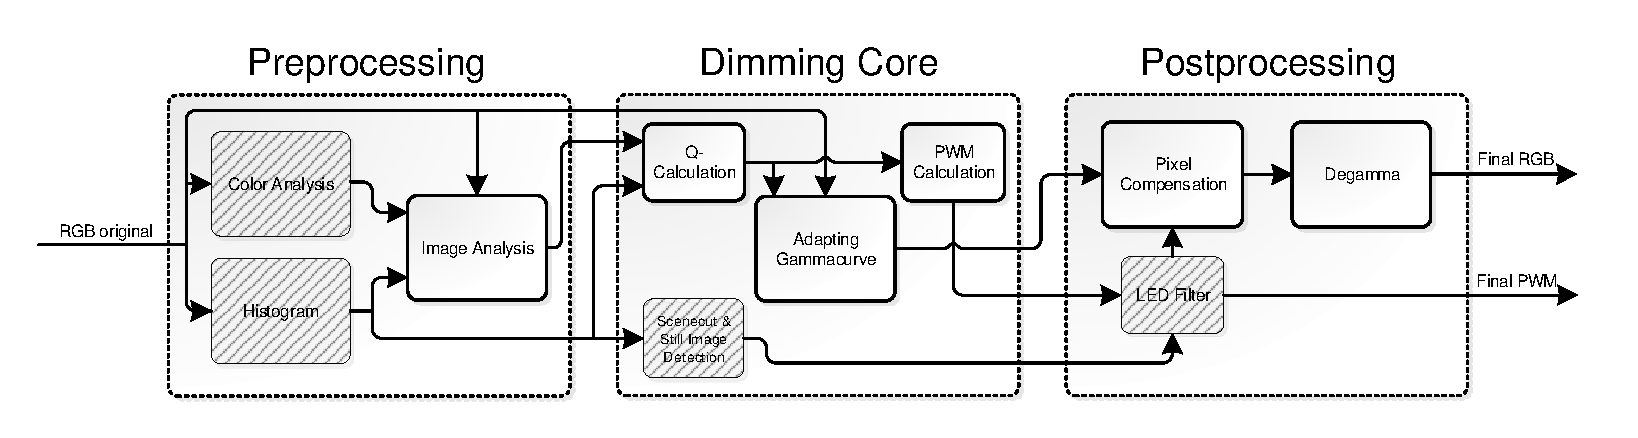
\includegraphics[width=1\linewidth]{img/display_projekt/0D_basics/Blockdiagramm_Full}
	\caption[Blockdiagramm eines Global-Dimming Algorithmus]{Blockdiagramm und Datenfluss eines am \emph{LME} entwickelten Global-Dimming Algorithmus \cite{Schmidt_edC16}}
	\label{fig:dimming_block_full}
\end{figure}

\subsubsection{Vereinfachung des Algorithmus}
Für das Praktikum kann ein Global-Dimming Algorithmus als Vereinfachung des obigen Algorithmus aus Abbildung \ref{fig:dimming_block_full} verwendet werden. Dazu wird in Abbildung \ref{fig:dimming_block_Lab} der vereinfachte Ablauf dargestellt. Aufgrund von Hardware und Zeitlimitierung (Praktikum) entfallen einige der Blöcke aus obiger Abbildung automatisch. So werden die in grau hinterlegten Blöcke (Abb. \ref{fig:dimming_block_full}) für das Praktikum nicht berücksichtigt. \\
Die \emph{Scenecut \& Still Image Detection} und der darauf aufbauende \emph{LED Filter} sind nur für bewegte Bilder (Video) notwendig um erforderliche Maßnahmen bei Szenenwechsel durchführen zu können. Unser Praktikumsdisplay ist jedoch nur für Standbilder ausgelegt. Das \emph{Histogram} und \emph{Color Analysis} entfallen ebenfalls zur Vereinfachung.
\label{subsub:vereinfachung_0D}
\begin{figure}[H]
	\centering
	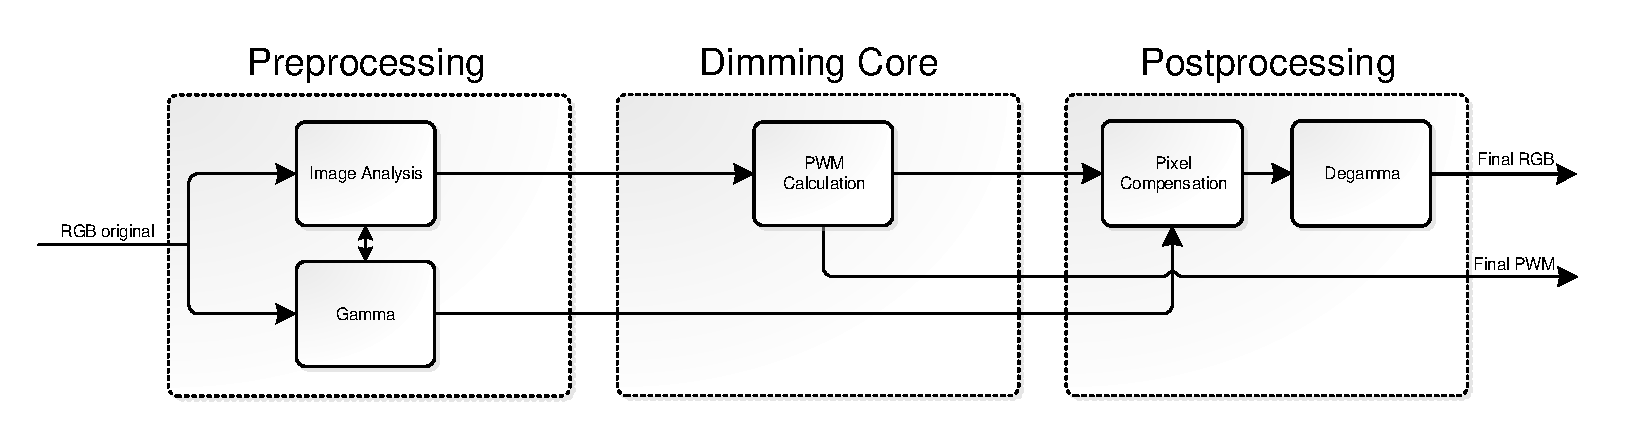
\includegraphics[width=1\linewidth]{img/display_projekt/0D_basics/Blockdiagramm_Lab}
	\caption{Blockdiagramm und Datenfluss eines vereinfachten Global-Dimming Algorithmus}
	\label{fig:dimming_block_Lab}
\end{figure}
Der vereinfachte Ablauf sieht keine Gammamanipulation wie in \ref{subsub:SoA_0D} beschrieben vor. Es wird folglich auch kein Knickpunkt bestimmt. Stattdessen soll eine Bildanalyse im \emph{Image Analysis} Block durch beispielsweise das Berechnen des maximalen Pixelwertes im Bild zur Berechnung des LED-Wertes beitragen.  Die Funktion der Pixelkompensation wie in Formel \ref{eq:compensation} beschrieben, bleibt erhalten. Ebenso das \emph{Degamma}. Die Ausgabe des Algorithmus sind der globale PWM-Wert sowie die kompensierten RGB-Werte. \\
Wie bereits weiter oben beschrieben, soll in einer konkreten Realisierung auf einen Frame-Buffer verzichtet werden. Dadurch werden nicht nur Kosten (SRAM) gespart, sondern auch nur ein minimales Delay verursacht, sodass der Algorithmus sich ohne Weiteres direkt in die vorhandene Pixelpipeline integrieren ließe. Im Praktikum wird jedoch wie bereits in \ref{subsec:Display_Beschreibung} beschrieben, ein SPI-Interface zur Übertragung der Bilddaten zum TCON des Displays verwendet. Aus diesem Grund wird nicht auf der eigentlichen Pixelclock (siehe \ref{subsec:display_timing}), sondern auf der Systemclock des FPGA Boards gearbeitet. Eine Pixelpipeline wird durch bestimmte Signale realisiert, die ein Pixelwechsel anzeigen. Siehe dazu Kapitel \ref{subsub:spezifizierung_dimming_modul}. Im Folgenden wird auf die konkrete Realisierung und Implementierung des Algorithmus im FPGA eingegangen. 
\subsection{Modulbeschreibungen und Spezifizierung}
\label{subsec:modulbeschreibung_und_spec}
Nachdem der Global-Dimming Algorithmus im vorangegangen Kapitel erläutert wurde, wird ein Überblick über die wichtigsten Module und deren Datenfluss bzw. Interaktion vorgestellt. Zunächst wird die gegebene Struktur beschrieben.


\subsubsection{Beschreibung der gegebenen Module}
\label{subsubsec:Beschreibung_vorhandenes_Verilog_Modul}
Wie bereits in Kapitel \ref{subsec:Display_Beschreibung} erwähnt, wird ein Grundgerüst zur Verfügung gestellt um den Aufwand während des Praktikums zu reduzieren. Aus Kapitel \ref{subsec:datenuebertragung} ist bereits die grobe Funktionsweise der erzeugten Pixel-Pipepline mit Hilfe des Bytestreams, sowie die Kommunikation mit dem Display-Controller bekannt.\\
Die in diesem Stream gesendeten Daten werden im FPGA an den speziellen EPP-Pins entgegengenommen. Um die Daten aus diesem Protokoll auslesen zu können, wird ein spezielles Modul integriert, welches jedes Mal, wenn ein neuer Datensatz anliegt ein Flag-Signal setzt, welches wiederum die weitere Verarbeitung dieses Signals im FPGA erlaubt. Die so angenommenen Daten werden nicht im FPGA gespeichert, sondern mittels eines weiteren speziellen Moduls über SPI zum Display geschickt. Hierbei liest eine State-Maschine die Codierung der LSBs im Stream aus (siehe Tabelle \ref{tab:bytestream}). Anhand dieser Information werden die RGB-Werte richtig zugeordnet. Durch ein Mitzählen der eingehenden Werte im Stream ist es auch möglich, die beiden erforderlichen Video-Boxen zu öffnen und auch die notwendigen Delay-Zeiten können ohne Problem eingehalten werden. All dies wird von der State-Machine direkt bei der ersten Übermittlung des ersten Wertes im Stream getriggert und läuft ab dann automatisch ab. \\
So wird auch zu Beginn eines jeden Bildes der Wert des Backlights eingestellt, dessen Funktion aus Kapitel \ref{sec:grundlagen_lcd} bereits bekannt ist. Dies führt beim Dimmen dazu, dass der Wert und auch die Kompensation der Pixelwerte erst beim zweiten Anzeigen des gleichen Bildes den richtigen Inhalt enthalten. Beim ersten Übertragen eines Bildes wird das Backlight immer zu 100\ \% eingeschaltet.

Ein Blockschaltbild des FPGA-Designs ist in Abbildung \ref{fig:block_verilog_module} dargestellt. Die rot umrandeten Funktionsblöcke werden als ein Modul (Interface) bereitgestellt.
\begin{figure}[H]
\centering
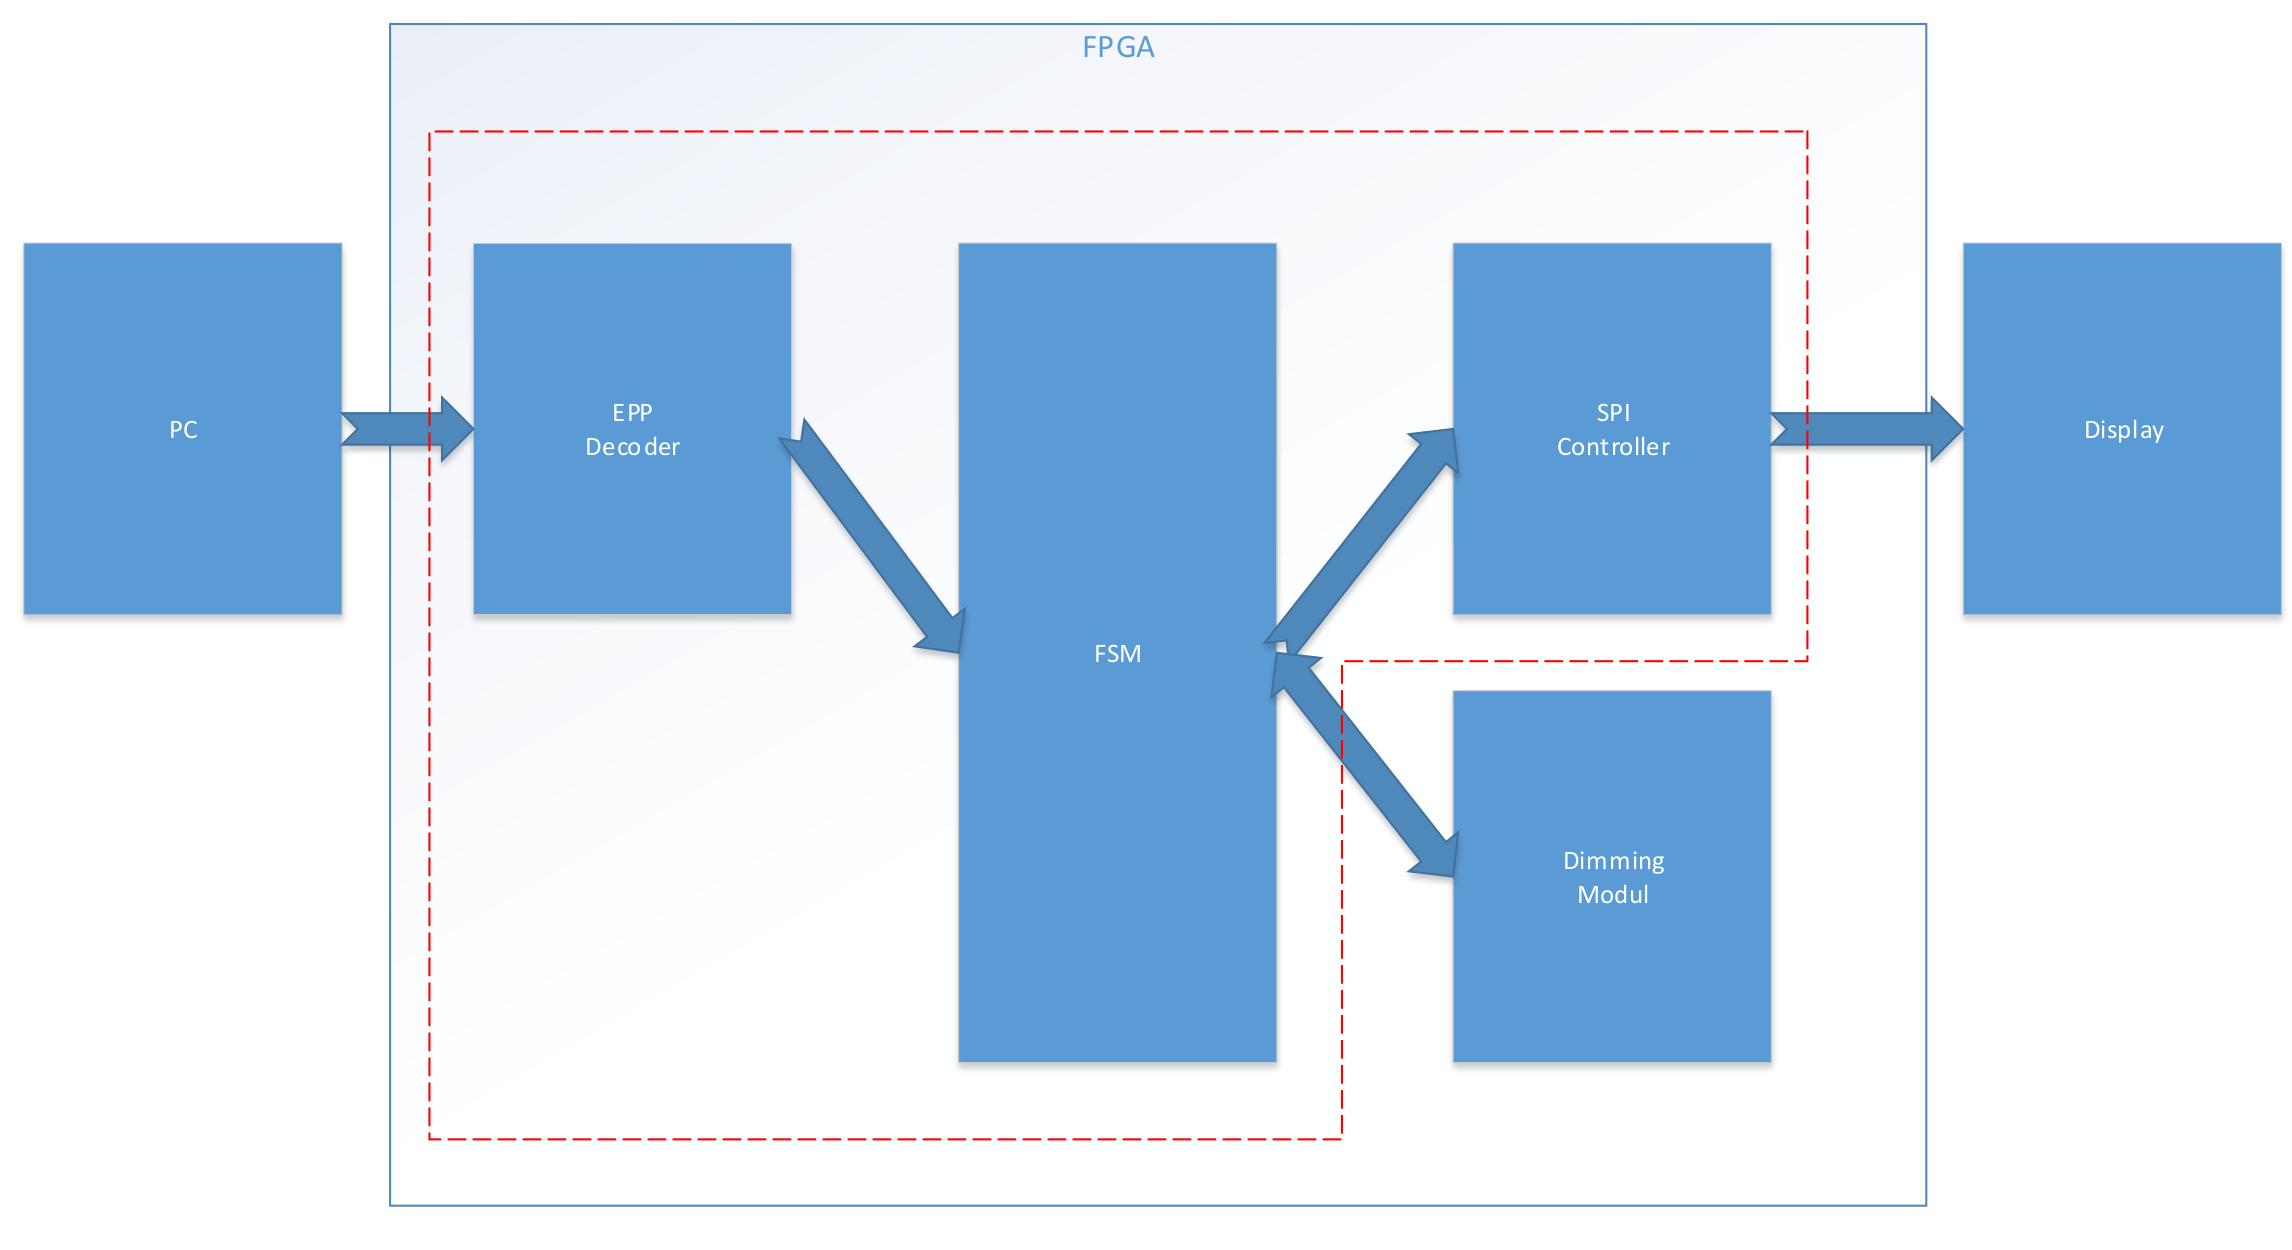
\includegraphics[width=1\linewidth]{img/display_projekt/Blockdiagramm_Module_gegeben}
\caption{Blockdiagramm und Datenfluss zwischen den einzelnen Funktionsblöcken}
\label{fig:block_verilog_module}
\end{figure}
Es ist auch in diesem Diagramm bereits ein \emph{Dimming-Modul} zu sehen. Dieses Modul kommuniziert ausschließlich mit der FSM im TOP-Modul. Das Dimming-Modul ermöglicht ein einfaches Manipulieren der Pixel-Werte und der Backlight-Werte. Im Folgenden wird näher auf das Dimming-Modul eingegangen. Der Algorithmus, welcher im Rahmen des Praktikums entwickelt wird, soll innerhalb dieses Moduls (inklusive weiterer Untermodule) implementiert werden.

\subsubsection{Spezifizierung des Dimming-Moduls}
\label{subsub:spezifizierung_dimming_modul}
Das in Abbildung \ref{fig:block_verilog_module} bereits aufgeführte Dimming-Modul wird im Folgenden näher beschrieben und spezifiziert. In der ausgelieferten Version unter\\
\texttt{\centerline{\netzwerkpfadSource/modules/dimming\_plain.v}}\\
fungiert das Modul als sogenanntes \emph{Durchschleifmodul}, um die ankommenden Bilddaten ohne Manipulation von den Eingängen zu den Ausgängen des Moduls zu schieben, es hat keine spezielle Funktion und soll für die folgenden Aufgaben erweitert werden. In der folgenden Abbildung sind die Ein- und Ausgänge des Moduls dargestellt.

\begin{figure}[H]
\centering
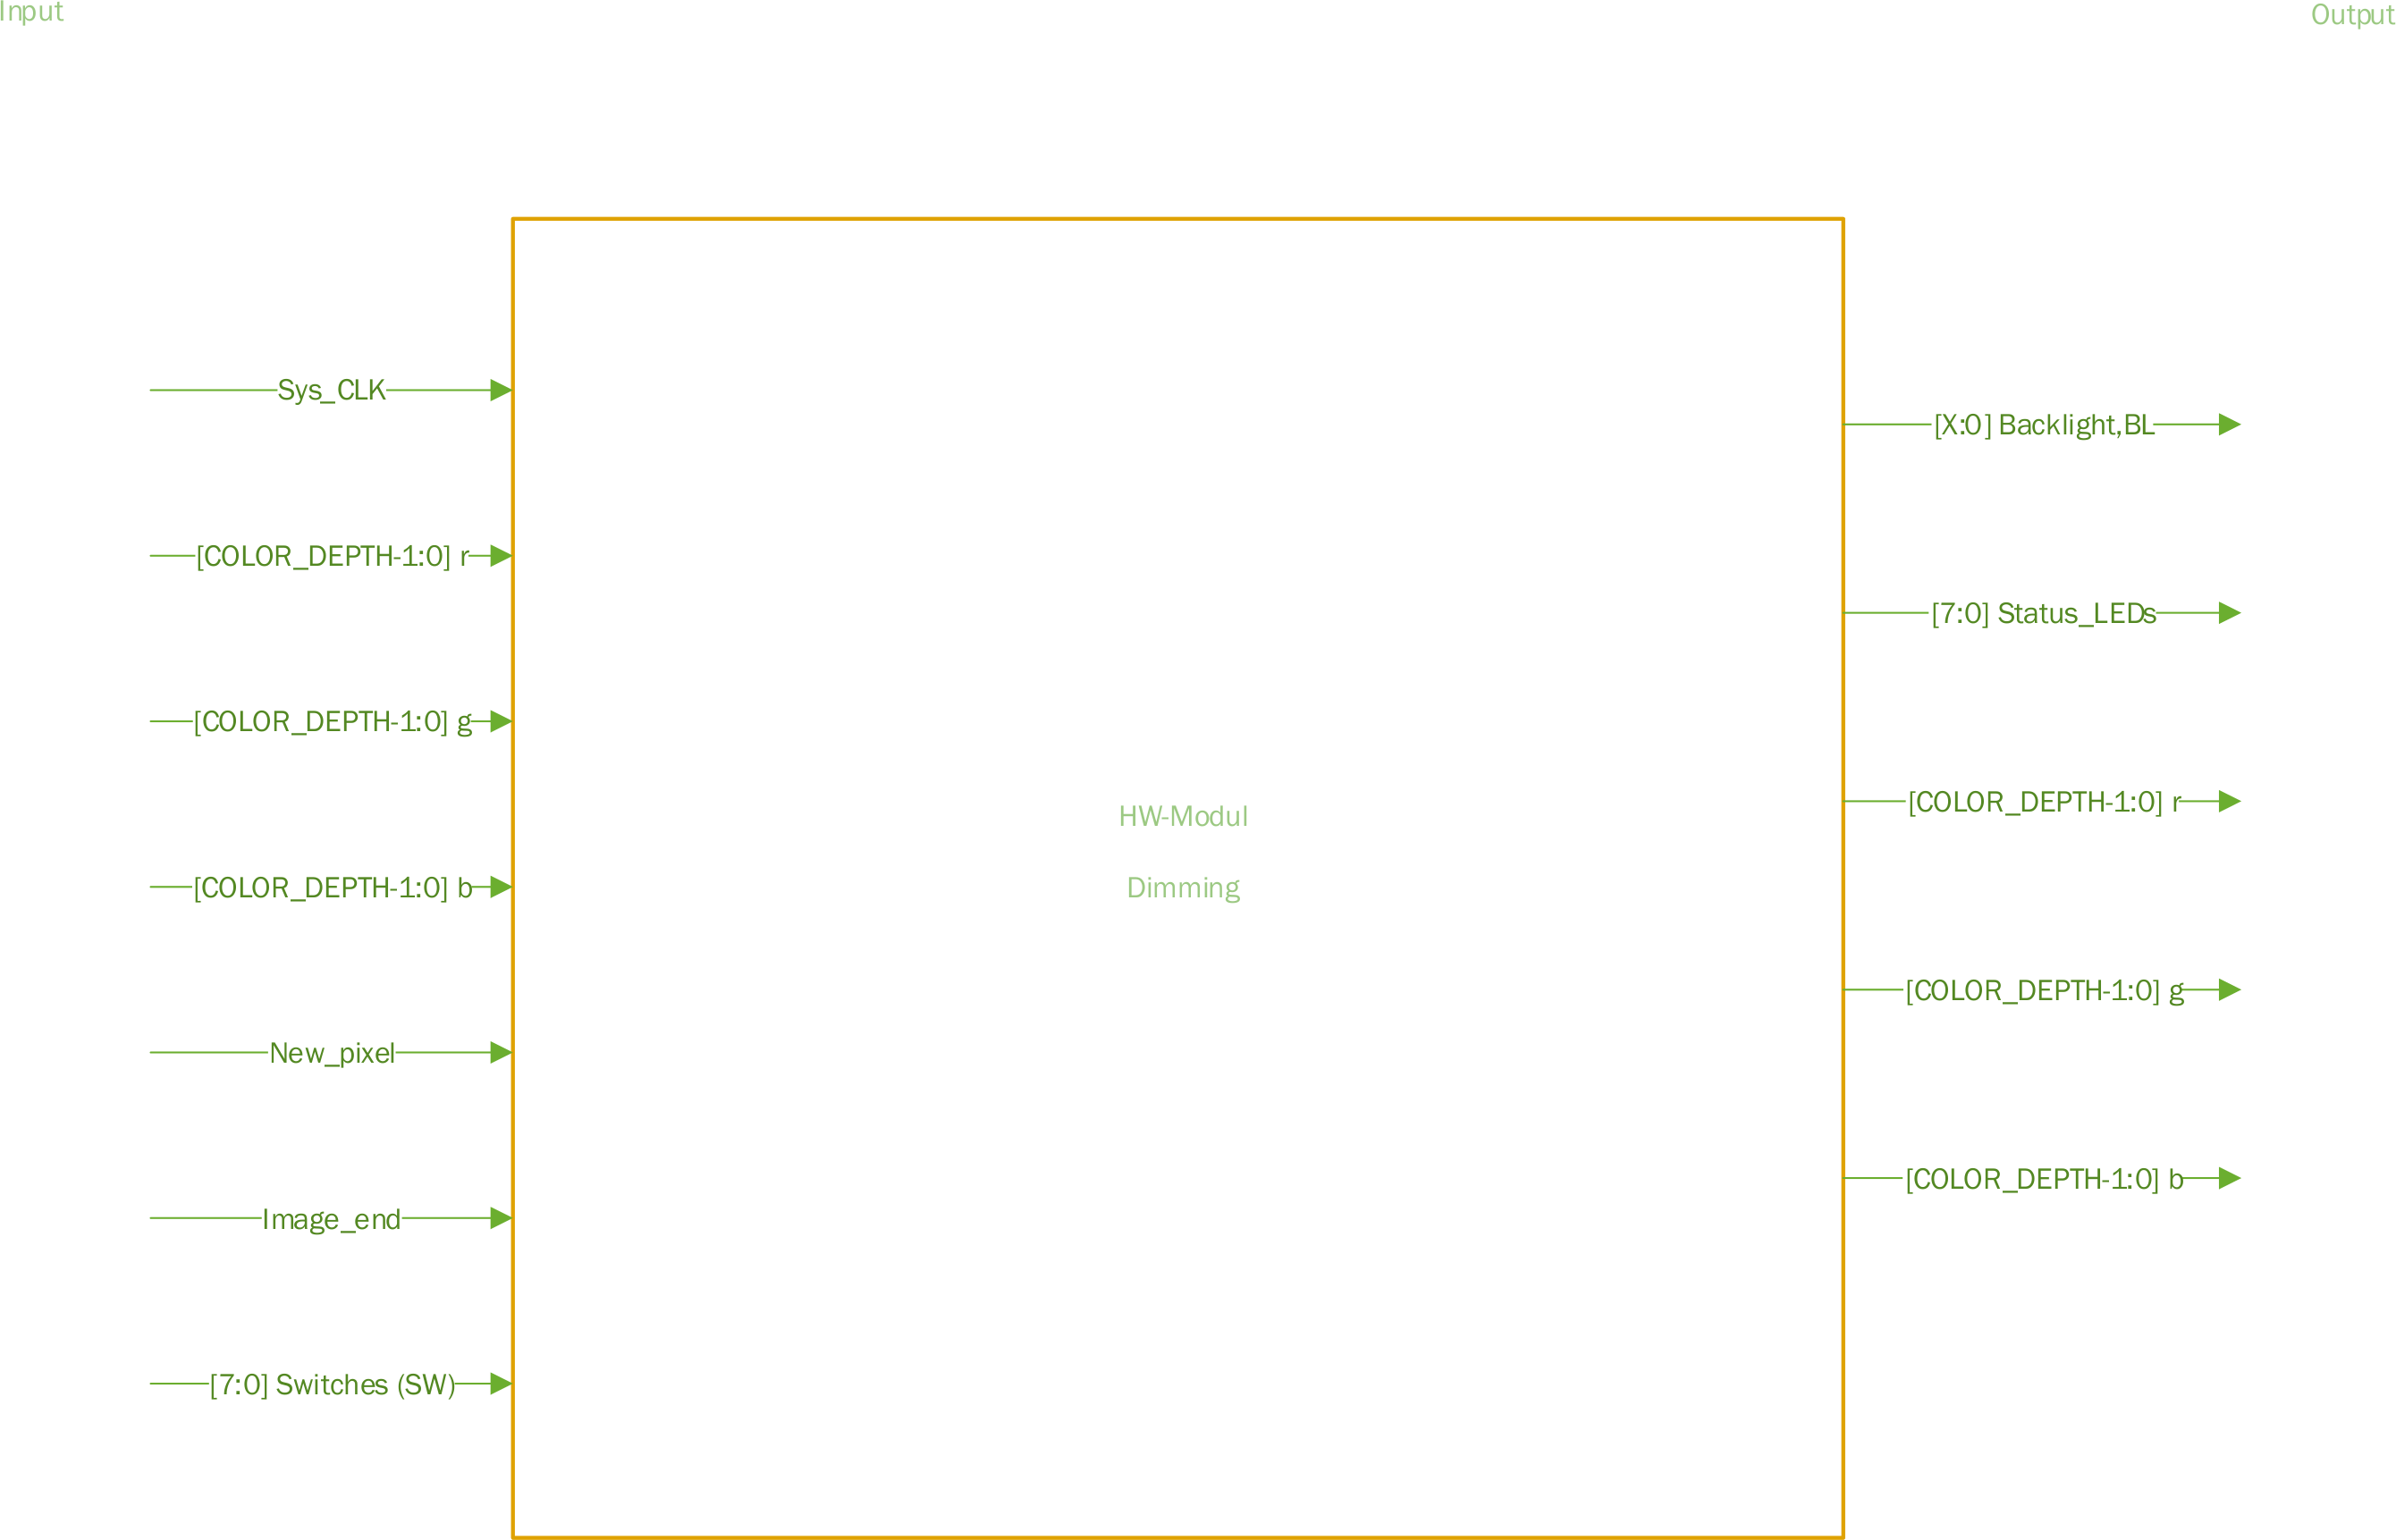
\includegraphics[width=0.9\linewidth]{img/display_projekt/Modul_HW_dimming}
\caption{Ein- und Ausgänge des Dimming-Moduls}
\label{fig:dimming_modul_portliste}
\end{figure}
Anhang der obigen Abbildung ist erkennbar, dass auch Backlight-Werte ausgegeben werden. Zunächst ist ein vorgegebener Wert im Modul selbst in einem Register gespeichert. Außerdem ist es zum einfachen Debuggen möglich die Schiebeschalter am Board zu nutzen und auch mit diversen Signalen die Status LEDs anzusteuern.\\
In Kapitel \ref{subsec:pipelining} wurde bereits der Begriff und Funktion des \emph{Pipelinings} eingeführt und in Kapitel \ref{subsec:display_timing} auf die Pixel-Pipeline transferiert. Da in diesem Praktikum die \emph{Systemclock} deutlich höher getaktet ist als die generierte Pixelclock, kann auf die Verwendung von komplexeren gepipelineten Multiplizierer und Dividierer verzichtet werden, da ausreichend viele Systemclock-Zyklen für die Berechnungen mit den RGB-Daten zur Verfügung stehen. D.h. die gesamte Logik soll mit der Systemclock -anstelle der Pixelclock- getaktet werden. Zu diesem Zweck, besitzt Ihr Modul einen \texttt{Sys\_CLK} Eingang und einen \texttt{New\_Pixel} Eingang, welcher ein neues Pixel signalisiert.\\
Wenn die Bilddaten modifiziert werden, ist darauf zu achten, dass das in der folgenden Abbildung gezeigte Timing eingehalten wird.
\begin{figure}[H]
\centering
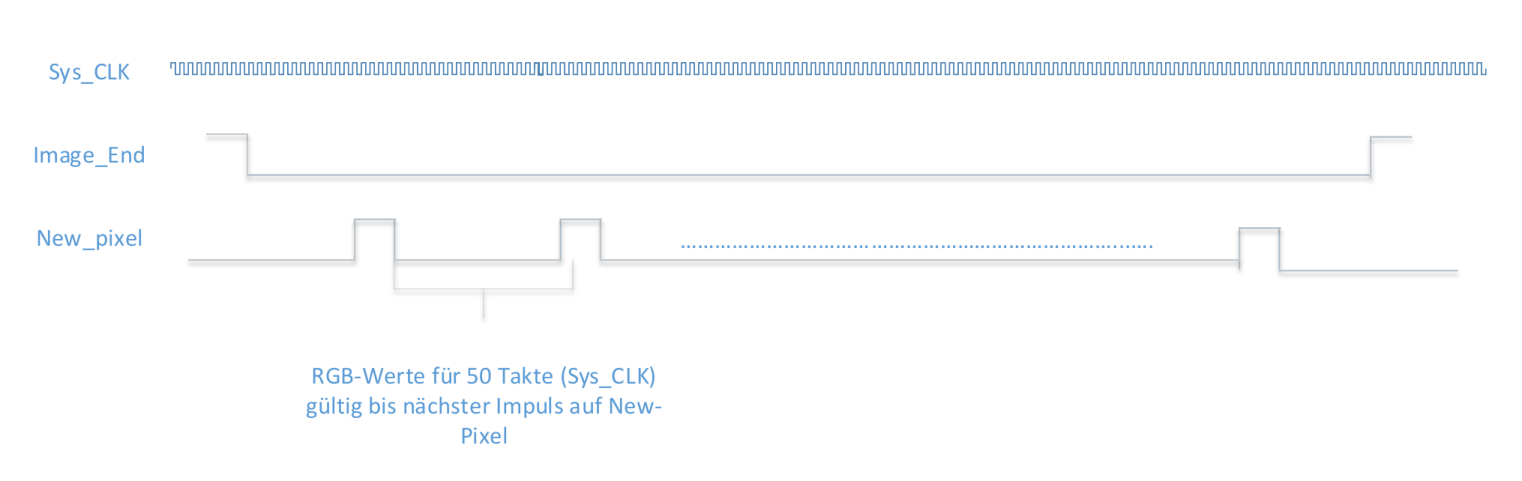
\includegraphics[width=1\linewidth]{img/display_projekt/zeitlicher_Ablauf}
\caption{Timing des Dimming-Moduls}
\label{fig:Timing_Dimming_Modul}
\end{figure}
Um das Timing zwischen der System- und virtuellen Pixelclock zu synchronisieren, erhält das Dimming-Modul das Signal \texttt{Image\_End} zusätzlich zu \texttt{New\_Pixel}. Bei steigender Flanke von \texttt{New\_Pixel} liegt am Eingang des Moduls ein neuer Pixelwert an. Der nächste Pixel folgt dann in mindestens 50 Takten (Sys\_clk) Abstand. Das heißt, sie haben 50 Takte lang Zeit die Pixelwerte zu manipulieren und am Ausgang des Moduls wieder bereit zu stellen. 
Ähnliches gilt für den berechneten Wert des Backlights. Dieser muss spätestens 15 Takte nach der steigenden Flanke von \texttt{Image\_End} anliegen. Wie bereits oben beschrieben wird der berechnete Backlight-Wert aber erst beim Anzeigen des nächsten Bildes verwendet. 

\subsubsection{Ein ROM-Modul}
\label{subsub:ROM-modul}
Im Folgenden ist die Verilog Beschreibung eines ROM Moduls beschrieben. Dieses Modul ist parametrisierbar. Machen Sie sich mit der Funktion dieses Moduls durch eine Simulation vertraut!
Die Daten können in Matlab generiert und in einer \texttt{*.coe} Datei gespeichert werden. Nutzen Sie dazu die Matlab Funktionen \texttt{fprintf()} und \texttt{dec2bin()}. Ein Beispiel für den Inhalt solch einer Datei ist unter dem ROM-Modul dargestellt.
\begin{figure}[H]
\lstset{style=verilog-style}
\begin{lstlisting}
module ROM #(
	parameter ROM_PATH = "PATH_TO_COE",
	parameter DATA_WIDTH = 10,
	parameter ADDR_WIDTH = 12,
	parameter LAST_ADDR = 4095)
	(
	input clk, 
	input [ADDR_WIDTH - 1:0] addr,
	output reg [DATA_WIDTH - 1:0] dout
	);

// LUT
reg [DATA_WIDTH - 1:0] rom [0 : LAST_ADDR];
  
initial $readmemb(ROM_PATH, rom, 0, LAST_ADDR ); 

always @ (posedge clk)  
    dout <= rom[addr];

endmodule
\end{lstlisting}
\caption{Ein ROM-Modul in Verilog}
\end{figure}
\begin{figure}[H]
\lstset{style=matlab-style}
\begin{lstlisting}
00000000
00000001
00000010
00000011
00000100
00000101
00000110
00001100
00001101
00001110
00001111
\end{lstlisting}
\caption{Beispielhafter Inhalt einer \texttt{*.coe} Datei}
\end{figure}
\subsection{\textsc{Versuch 4 und Aufgaben}}
Für den weiteren Ablauf sind die bereits einführten Module vorgegeben. In Abbildung \ref{fig:display_schematic_top_top} ist das Topmodul als Block dargestellt, dessen Ports direkt mit den FPGA-Pins verbunden sind. Der Verilog Code ist in der Datei \texttt{Top\_Module\_with\_Interface\_plain.v} in dem Ordner \\
\texttt{\centerline{\netzwerkpfadSource/modules/}}\\
zu finden. Die übrigen benötigte Module, wie der Rumpf des Dimming-Moduls (\texttt{dimming\_plain.v}) befinden sich ebenfalls im zuvor genannten Ordner.
\begin{figure}[H]
\centering
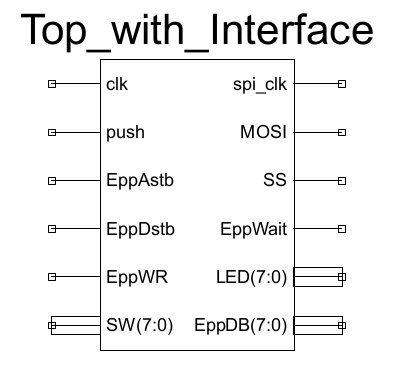
\includegraphics[width=0.3\linewidth]{img/display_projekt/top_schematic}
\caption{Blockdarstellung des Topmoduls mit IOs.}
\label{fig:display_schematic_top_top}
\end{figure}
In der Abbildung \ref{fig:display_schematic_interface_dimming} wird die Verbindung zwischen dem Kommunikationsinterface und dem Dimming-Modul abgebildet. Das Instantiation-Template des enthaltenen Dimming-Moduls ist in Abbildung \ref{code:instantiation_dimming} dargestellt.

\begin{figure}[H]
\lstset{style=verilog-style}
\begin{lstlisting}
parameter COLOR_DEPTH = 2;
parameter DEFAULT_BL_VALUE = 255;

dimming_durchschleif
 #(.COLOR_DEPTH(COLOR_DEPTH), .DEBUG_BL_VALUE(DEFAULT_BL_VALUE))  
    dimming_durchschleif_modul (
    .clk(clk),
    .r(R_in), 
    .g(G_in),
    .b(B_in),
    .new_pixel(new_pixel),
    .image_end(image_end),
    .SW(SW),
    .r_out(R_out),
    .g_out(G_out),
    .b_out(B_out),
    .BL(BL),
    .LED(LED_from_Dimming) // status LEDs
);
\end{lstlisting}
\caption{Instantiation Template des Dimming-Moduls}
\label{code:instantiation_dimming}
\end{figure}
\begin{figure}[H]
\centering
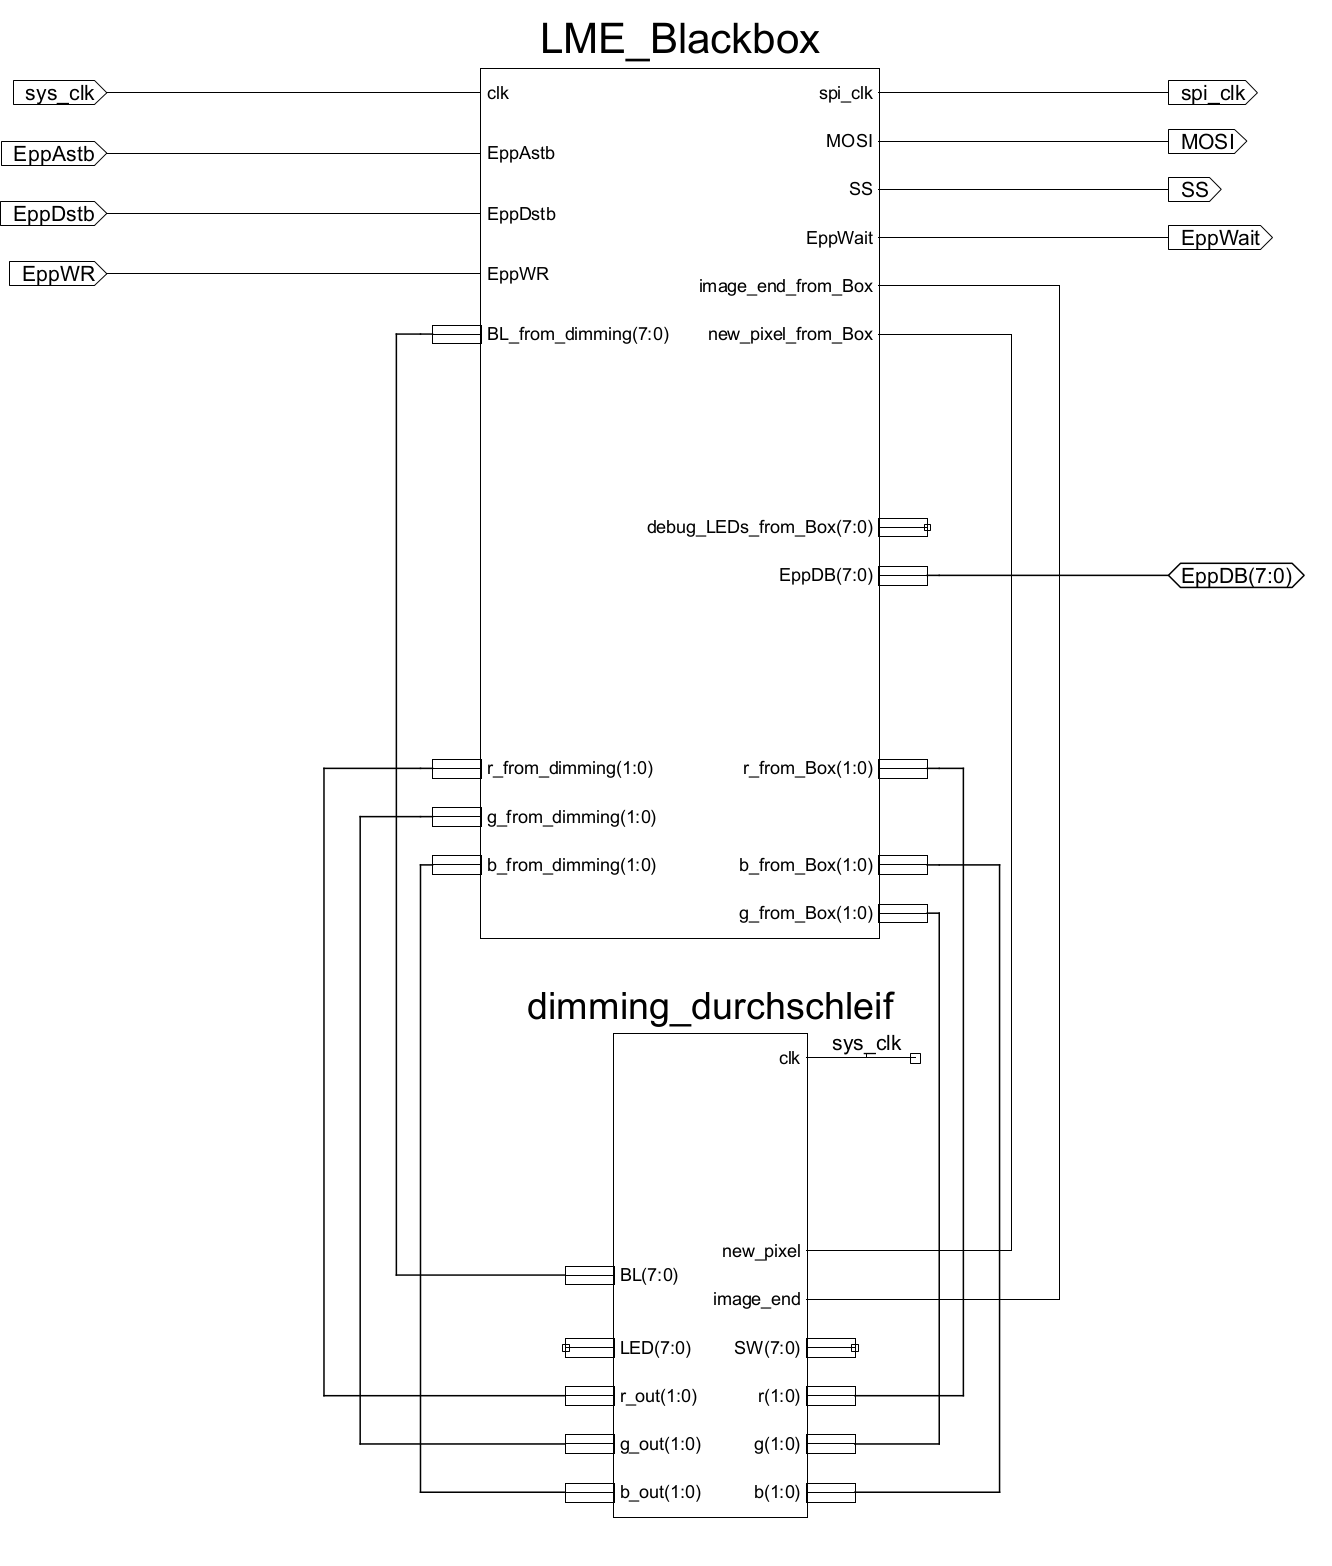
\includegraphics[width=0.8\linewidth]{img/display_projekt/schematic_interface_dimming}
\caption{Verschaltung zwischen dem Kommunikations-Interface und Dimming-Modul.} 
\label{fig:display_schematic_interface_dimming}
\end{figure}
\textbf{Die Aufgaben sind im Dokument zur Aufgabenstellung in Kapitel 4 zu finden.}
